\subsection{Salade niçoise}

% source: https://www.colruyt.be/fr/en-cuisine/recette/salade-nicoise

\culabel{salade-nicoise}{4}

\begin{center}
	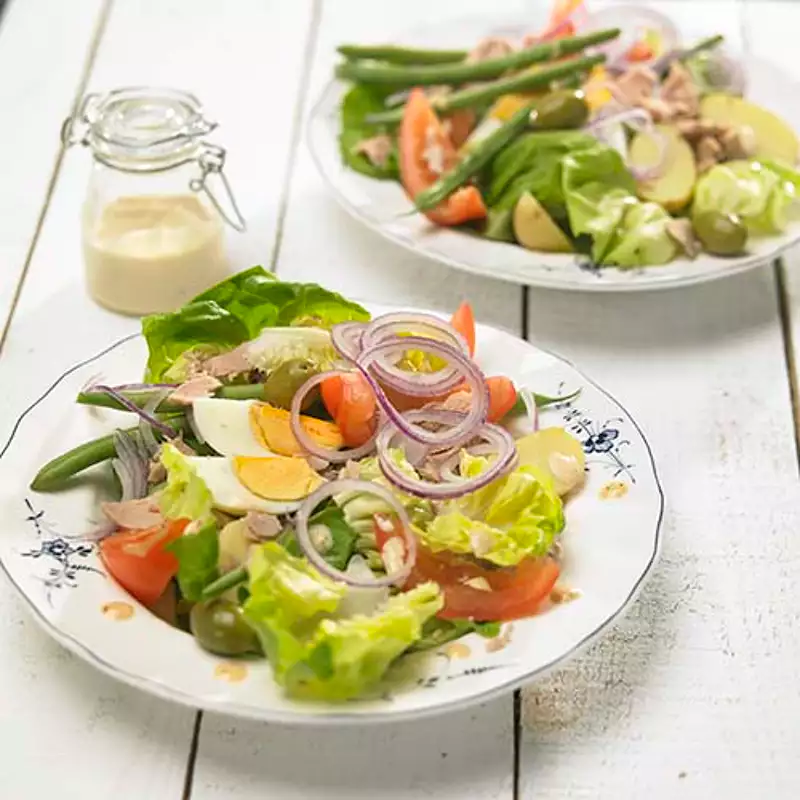
\includegraphics[trim={0 0 0 0},clip,height=3cm,width=0.8\linewidth]{./img/salade-nicoise.png}
\end{center}


\subsubsection*{À propos}

\begin{center}
	\begin{tabularx}{0.8\linewidth}{|c|X|c|c|} \hline
		Type & Temps & Pour & Matériel \\ \hline
		Plat & 40 minutes (25 minutes + temps de refroidissement) & \curef{salade-nicoise} personnes & \Gasstove \\ \hline
	\end{tabularx}
\end{center}


\subsubsection*{Ingrédients}

\begin{multicols}{2}
	\begin{itemize}
		\item Haricots verts \cunum<salade-nicoise>{250}{g} \index{Haricot vert}
		\item Tomates \cuam<salade-nicoise>{3} \index{Tomate}
		\item Laitue \cuam<salade-nicoise>{1} \index{Laitue}
		\item Grenailles \cuam<salade-nicoise>{8} \index{Grenaille}
		\item Oignon rouge \cuam<salade-nicoise>{1} \index{Oignon rouge}
		\item Olives vertes Picholine \cunum<salade-nicoise>{100}{g} \index{Olive}
		\item Oeufs \cuam<salade-nicoise>{4} \index{Oeuf}
		\item Thon au naturel (boîte) \cunum<salade-nicoise>{200}{g} \index{Thon}
		\item Mayonnaise \cunum<salade-nicoise>{2}{EL} \index{Mayonnaise}
		\item Moutarde \cunum<salade-nicoise>{1}{EL} \index{Moutarde}
		\item Vinaigre de vin rouge \cunum<salade-nicoise>{1}{TL} \index{Vinaigre de vin}
		\item Poivre noir
		\item Sel
	\end{itemize}
\end{multicols}


\subsubsection*{Préparation}

\begin{enumerate}
	\item Lavez soigneusement les grenailles non pelées sous l'eau froide.
	Faites-les cuire \cutext{20}{min} dans de l'eau bouillante légèrement salée.
	Égouttez et laissez complètement refroidir.
	\item Entre-temps, faites cuire les oeufs \cutext{10}{min} dans de l'eau bouillante.
	Laissez-les refroidir, écalez-les et coupez-les en quartiers.
	\item Faites cuire les haricots verts \cutext{7--8}{min} à découvert dans de l'eau bouillante légèrement salée.
	Égouttez-les et passez-les sous l'eau froide.
	\item Entre-temps, détaillez l'oignon rouge en fines rondelles et les tomates en quartiers.
	Épépinez les tomates.
	Détachez les feuilles de laitue.
	\item Mélangez la mayonnaise avec la moutarde et le vinaigre de vin rouge.
	Salez et poivrez.
	\item Égouttez le thon et morcelez-le.
	\item Mélangez les haricots verts avec les grenailles, le thon, les oeufs et les tomates.
	Ajoutez les olives et le dressing à la moutarde.
	\item Déposez les feuilles de laitue sur les assiettes et répartissez la salade niçoise par-dessus.
	Parsemez de rondelles d'oignon rouge.
\end{enumerate}
